%!TEX root = ../thesis.tex

\section{Sweepcycle algorithm}
  \label{s:sweep}
  The first step of the algorithm is executing a sweepcycle algorithm comparable to Fusy's \cite{Fusy2006}. We will use a script $\C$ to indicate the current sweep cycle. With vertices $\pS, v_1 = \pW, v_2, \ldots v_{n-1}, v_n = \pE, \pS$.

  We will repeatedly only consider the path $\cpath$. In that case we will always order it from $\pW$ to $\pE$. That these edges are always in $\C$ is a result of Invariant \ref{i:uni:SWandSE}.

  We will let $\P$ denote a interior path. Given such a path of $k$ vertices we will index it's nodes by $p_1, \ldots, p_k$ in such a way that $p_1$ is closer to $\pW$ then $p_k$ is (and thus that $p_k$ is closer to $\pE$ then $p_1$ is). Given such a path the \emph{index} of a vertex $p_i\ in \P$ is it's position in the path, that is, the index of $p_i$ is $i$.

  Then $p_1$ and $p_k$ indicate the two unique vertices of the walk that are also part of the cycle. We will then let $\restC{\P}$ denote the part of $\cpath$ that is between $p_1$ and $p_k$ (including). $\C_\P$ will denote the cycle given by $\restC{\P} \oplus \rev(\P)$.

  During the algorithm we will want to maintain several invariants on $\C$. The first three are equivalent to those imposed by Fusy. The final invariants is new and will turn out to impose a nice structure on the sweepcycle so far.

  Before giving the invariant let us recall the Interior vertex condition: In the rotation around every vertex we have the following subsequent non-empty sets: Incoming red edges, incoming blue edges, outgoing red edges and outgoing blue edges.

  \begin{invariants}
    \itemsep=-4pt

    \item \label{i:uni:SWandSE} The cycle $\C$ contains the two edges $\pS \pW$ and $\pS \pE$.
    \item \label{i:uni:noChords} $\cpath$ has no chords
    \item \label{i:uni:intVertCond} All inner edges of $G$ in the exterior of $\C$ are colored and oriented such that the inner vertex condition holds for all vertices in the exterior of $C$.
    \item \label{i:uni:no2Chords} $\C\sm{\pS}$ has no separating 2-chords that don't use $\S$
  \end{invariants}

  \begin{defi}[Prefence]
    A prefence $\P$ is a interior path of $\C$ starting at $v_i \in \C$ and ending at $v_j \in \C$ a both adjacent to $\pS$
    \begin{enumerate}
      \itemsep=-4pt
      \renewcommand*{\labelenumi}{(P\arabic{enumi})}%
      \renewcommand*{\theenumi}{(P\arabic{enumi})}%

      \item  $\C_\P$ Has no interior vertex
      \label{p:noInteriorVertex}
      \item  $\P$ has no chords on the left     \label{p:Wchordfree}
      \item  The paths $v_1 v_2 \ldots v_i$ and $v_j v_{j+1} \ldots v_n$ have no chords nor 2chords on the right     \label{p:Cchordfree}
    \end{enumerate}
  \end{defi}

  Each update of the sweepcycle consists of the following three steps do the following
  \begin{enumerate}
    \itemsep=-4pt
    \item Take the right neighbor walk
    \item Evade irregularities on this path
    \item Update the sweepcycle with this path
  \end{enumerate}

  We then repeat this until the sweepcycle does not contain any more interior vertices. At which point we can terminate the algorithm by coloring the edges still on the cycle blue and its interior edges red.

  \paragraph{Find the right neighbor path}
    Let $v_i$ denote all the vertices of $\cpath$ in the following order $\pW =  v_1 \  v_2 \  \ldots v_{n-1} \  v_n = \pE$.
    Some intervals of these vertices will be adjacent to $\pS$. However, they can't be all adjacent to $S$ since then any vertex still in the interior of $\C$ would lie in a separating triangle of $G$. We denote by $v_i$ the last vertex of first interval of vertices adjacent to $S$ and by $v_j$ the first vertex of the second interval.
    As candidate path we will take the right neighbor path of $\cpath|_{v_i, v_j}$.
    The current situation is also depicted in Figure \ref{fig:sweep:rightNeighbourwalk}.

    \begin{figure}[h]
      \centering
      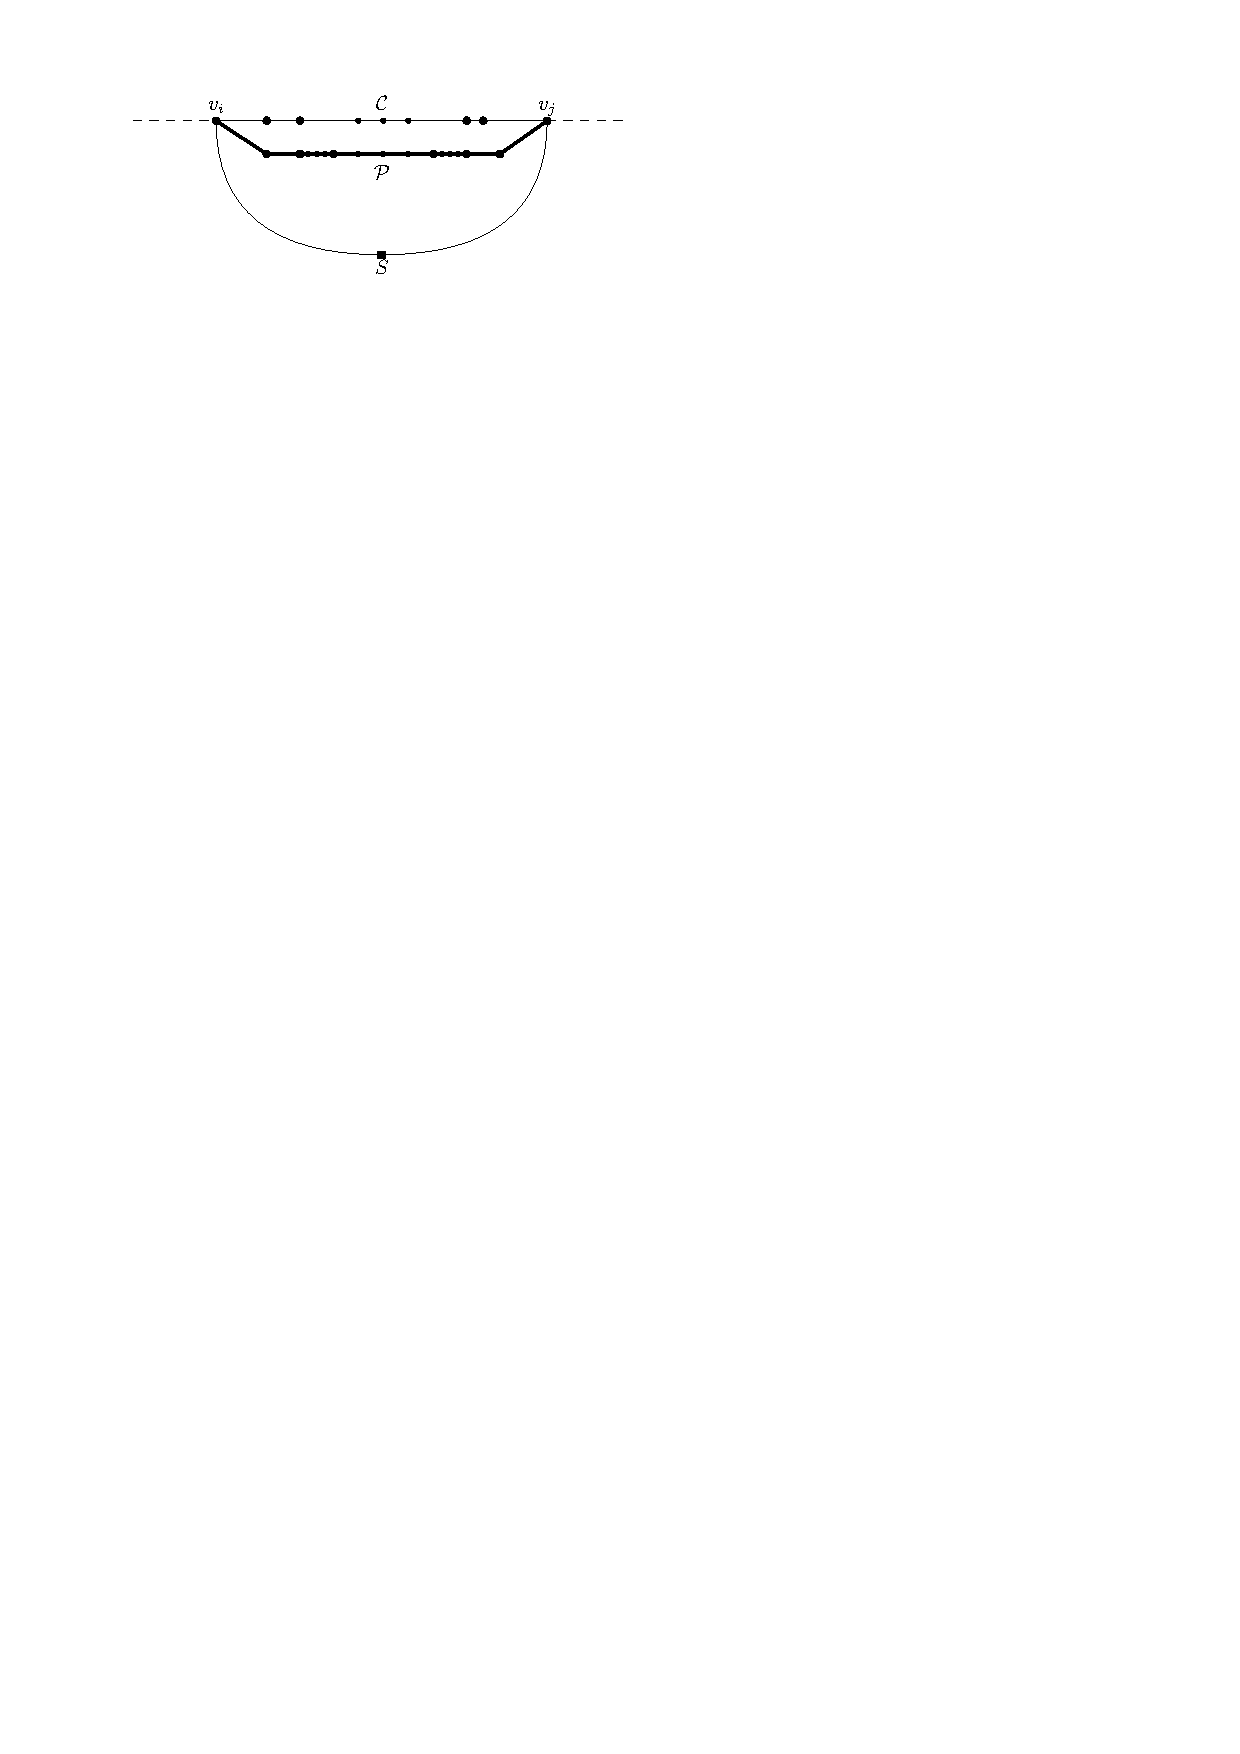
\includegraphics[scale=1]{unifiedAlgo/img/sweep/rightNeighbourWalk}
      \caption{}
      \label{fig:sweep:rightNeighbourwalk}
    \end{figure}

    \begin{lemma}
      \label{lm:uni:isPrefence}
      The right neighbor path $\P$ of $\cpath|_{v_i, v_j}$ described above is indeed prefence.
    \end{lemma}
    \begin{proof}
      $\P$ is a walk by Lemma \ref{lm:uni:neighborWalk}. Furthermore it is a path since any non-simple point would offend Invariant \ref{i:uni:no2Chords} of the sweepcycle.


      We note \ref{p:noInteriorVertex} holds due to Lemma \ref{lm:uni:neighbourwalkNoInteriorVertex}

      We note \ref{p:Wchordfree} holds due to Lemma \ref{lm:uni:neighbourwalkChordFree}.

      We note \ref{p:Cchordfree} holds due to Invariants \ref{i:uni:noChords} and \ref{i:uni:no2Chords}.
    \end{proof}

    We then orient $\P$ from $v_i$ (the vertex closest to $\pW$)to $v_j$ (the vertex closest to $\pE$) and denote it's vertices by $w_1 \ldots w_k$.

  \subsection{Irregularities}
    Now the prefence we found can have several structures we want to avoid
    namely
    \begin{enumerate}
      \itemsep=-4pt
      \item Chords
      \item Separating 2-chords
    \end{enumerate}

    All of these structures are on the right of the prefence since the prefence satisfies \ref{p:Wchordfree} (no chords on the left) and \ref{p:noInteriorVertex} (no separating 2-chords on the left).

    The \emph{range} of an irregularity will be given by it's start and end index.

    \paragraph{We have no irregularity}
      When there are no irregularities we \emph{augument} the sweecyle with the prefence $\P$.

    \paragraph{We have any chord} \mbox{ }
    \fxwarning[nomargin, inline]{Why not just take the inner chord?}
    We know that we can't have any polebound chords on the prefence since any such chord would offend Invariant \ref{i:uni:no2Chords} of the sweepcycle.

    If our prefence has any chords we look identify the them by their start and end vertex. Of the chords with the lowest start index we will consider the one with the largest end index. Let's call this chord $C_\text{outer}$.

    We now consider $C_\text{outer}$ and any chord contained therein. In this collection we look for the chord $C_\text{inner}$ with the smallest range (i.e. highest start $i_0$ and lowest end $j_0$) then we find the chord $C_\text{final}$ with the largest range that still starts at $i_0$ or ends at $j_0$. We will denote the range of $C_\text{final}$ by $\braces{i_1, \ldots, j_1}$.

    The way in which these chords are chosen is illustrated in Figure \ref{fig:sweep:chordsOnPrefence}.

    \begin{figure}[h]
      \centering
      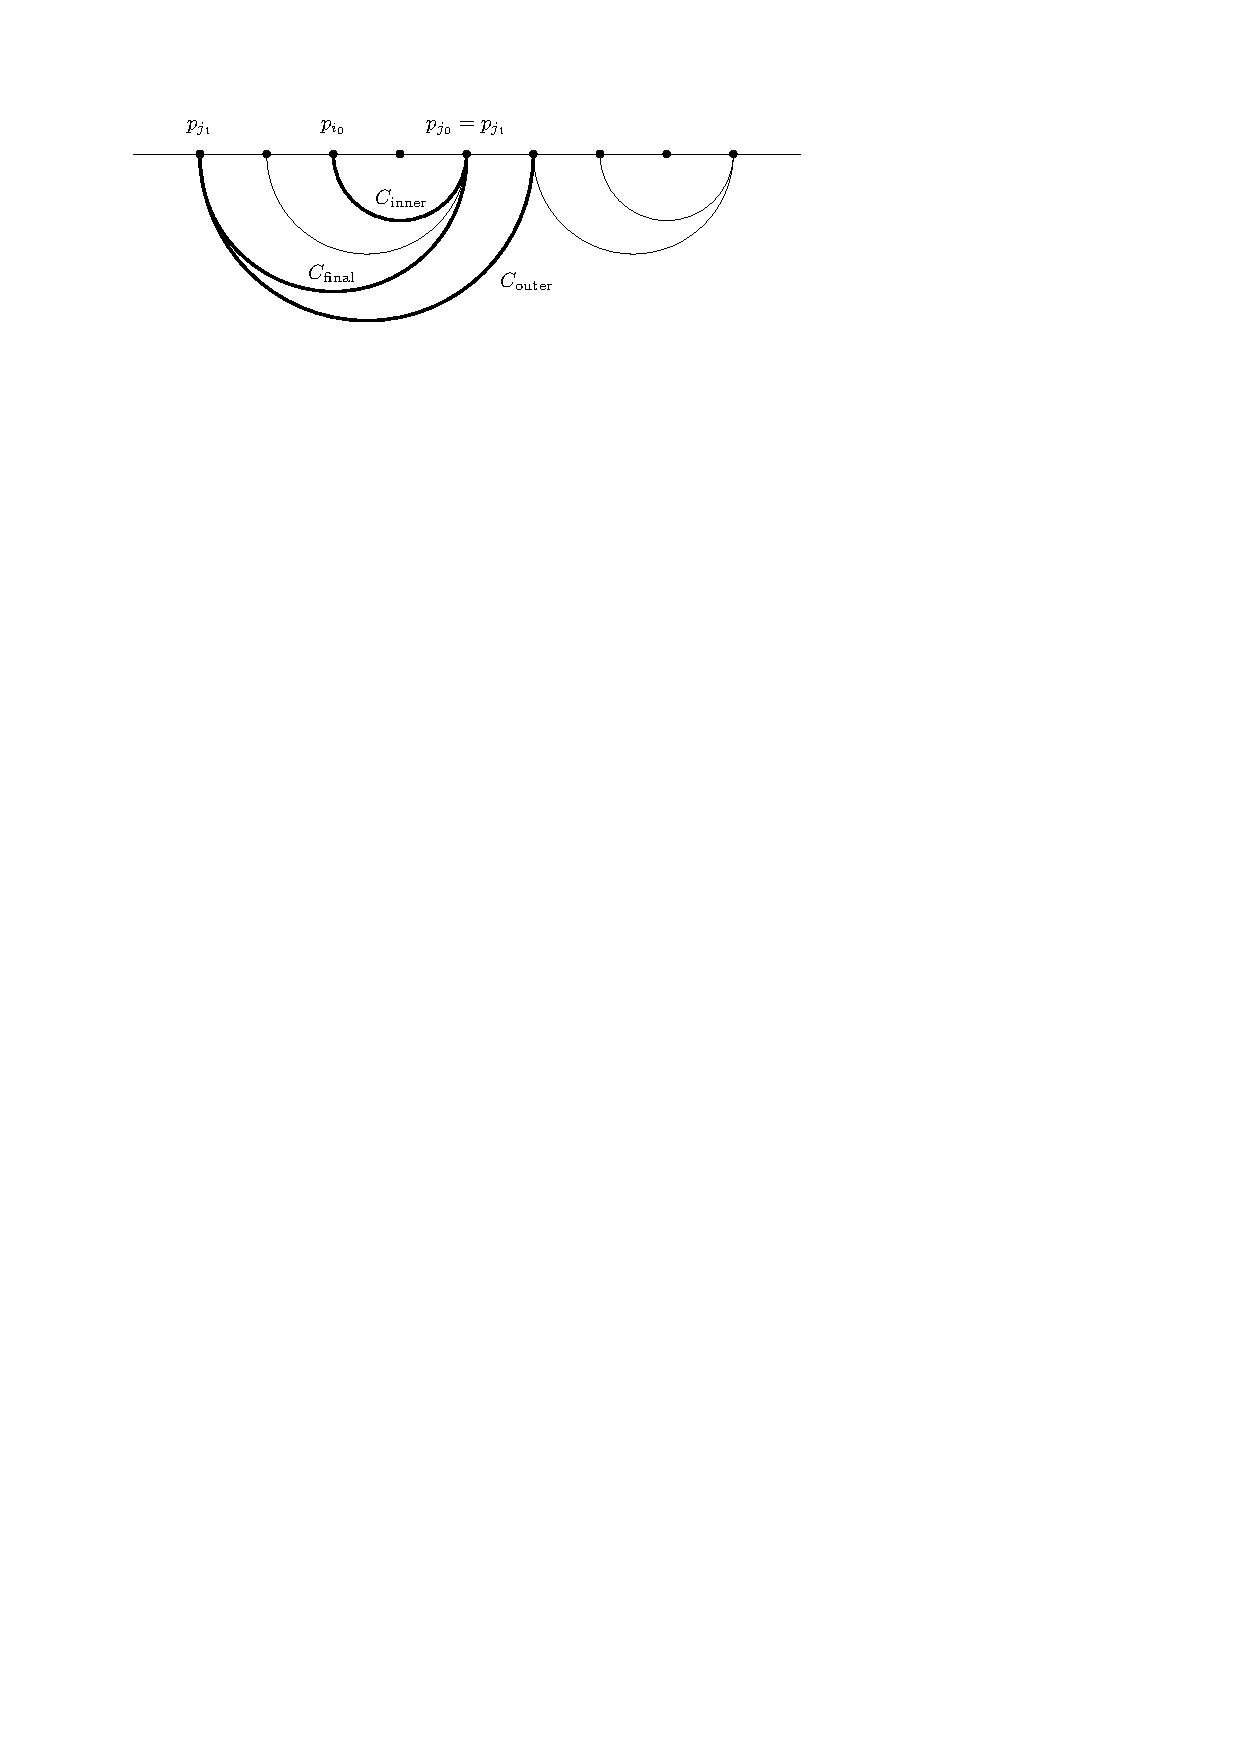
\includegraphics[scale=1]{unifiedalgo/img/sweep/chordsOnPrefence}
      \caption{}
      \label{fig:sweep:chordsOnPrefence}
    \end{figure}

    What we do now depends on whether a 2-chord shows up in the interior of the chord pasted to the prefence $\P|_{i_1, j_1} \oplus \rev({C_\text{final}})$.

    \fxwarning{Define augment, Take care of normal vertices and begin/end vertices- predraft 2}

    \emph{No separating 2-chord}
    If there is no separating 2-chord in the interior of $\P|_{i_1, j_1} \oplus \rev({C_\text{final}})$ we do the following. Let $v_k$ be the shared neighbor on the sweepcycle of $p_{i_1}$ $p_{i_1 +1}$ and $v_l$ the shared neighbor on the sweepcycle  of $p_{j_1 -1}$ and $p_{j_1}$. We augment the sweepcycle with the right neighbor path of $\cpath|_{v_k, v_l}$. See Figure \ref{fig:sweep:chordUpdate}.

    \begin{figure}[h]
      \centering
      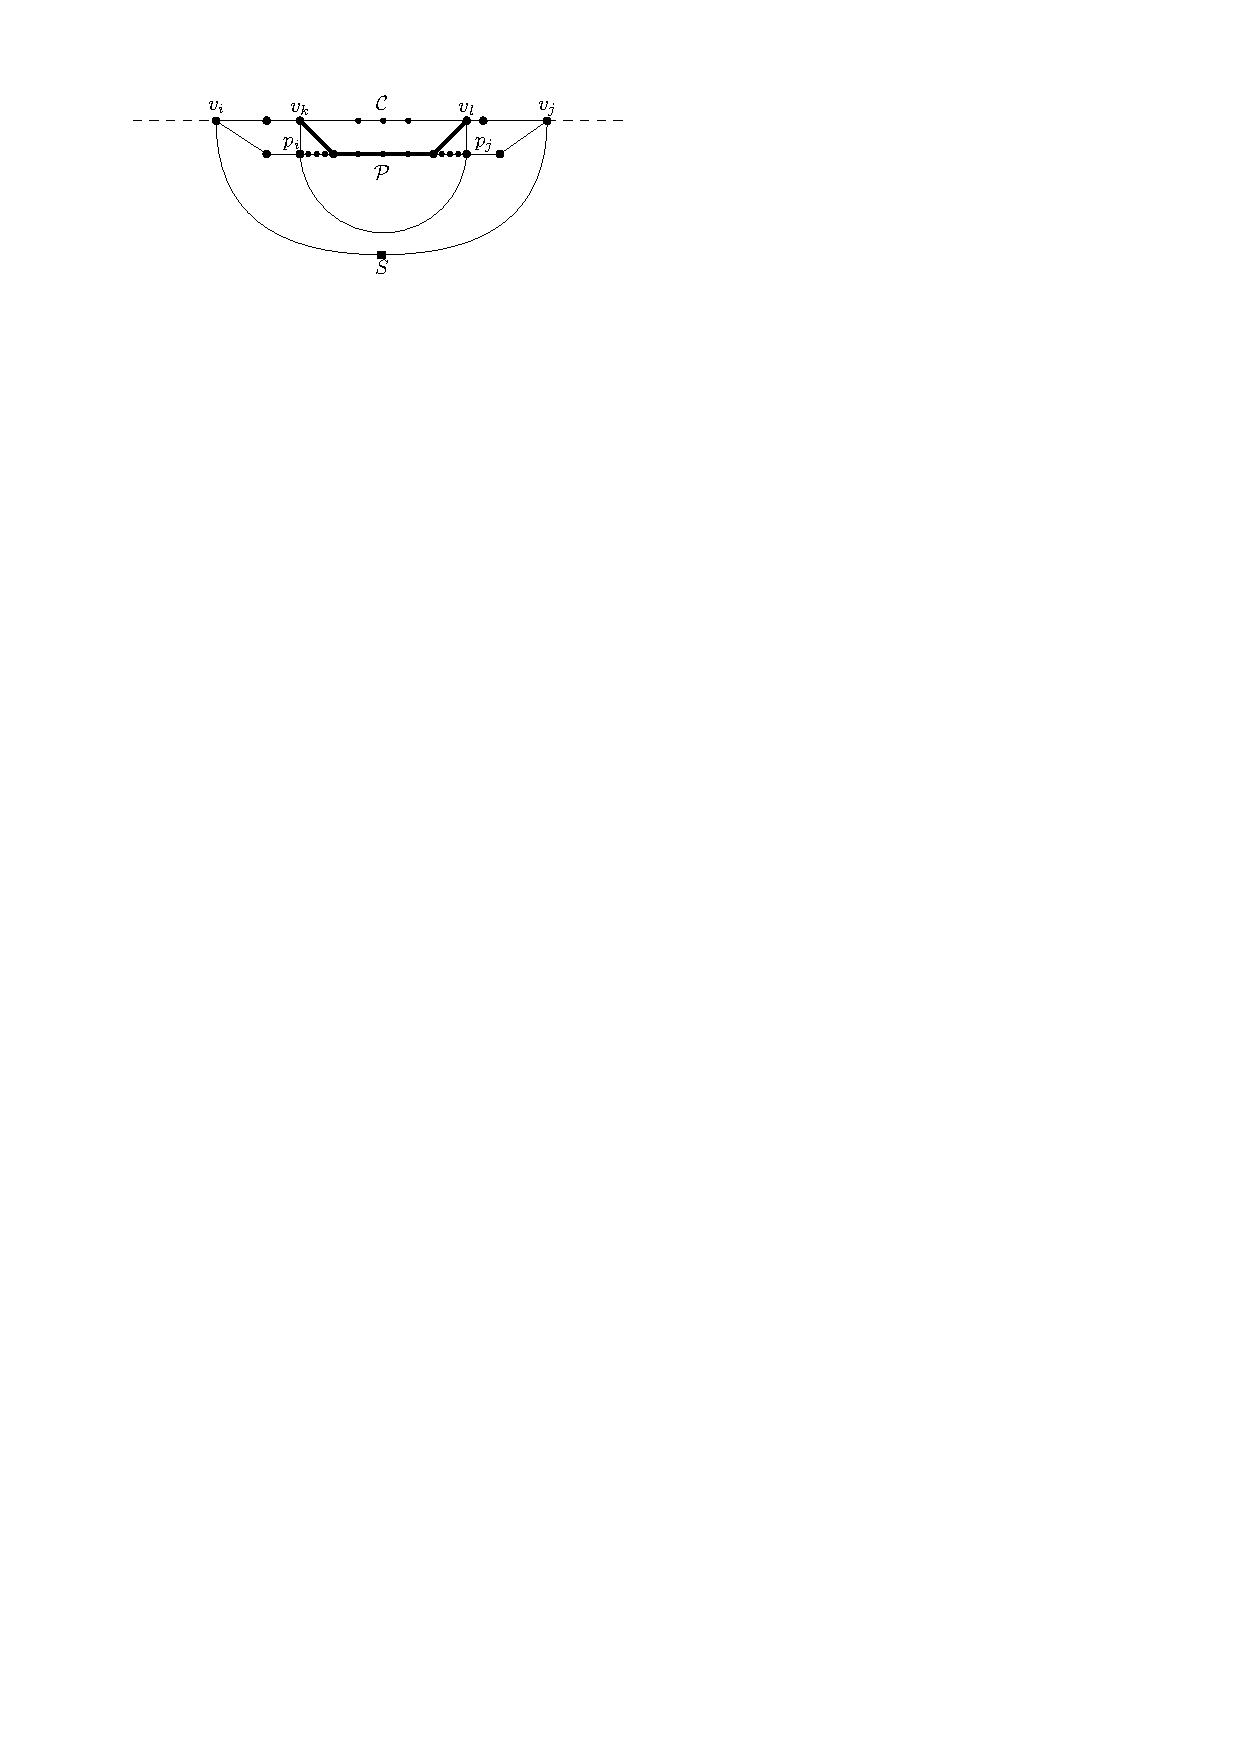
\includegraphics[scale=1]{unifiedAlgo/img/sweep/chordUpdate}
      \caption{}
      \label{fig:sweep:chordUpdate}
    \end{figure}

    \emph{A separating 2-chord}
      If separating 2-chord with the lowest end range in the interior of $\P|_{i_1, j_1} \oplus \rev({C_\text{final}})$ has end range $j_2$ then we augument the sweepcycle in the following way.

      Let $v_k$ be the shared neighbor on the sweepcycle of $p_{i_1}$ $p_{i_1 +1}$ and $v_l$ the shared neighbor on the sweepcycle  of $p_{j_2 -1}$ and $p_{j_2}$. We augment the sweepcycle with the right neighbor path of $\cpath|_{v_k, v_l}$. See Figure \ref{fig:sweep:2chordInChordUpdate}.

    \begin{figure}[h]
      \centering
      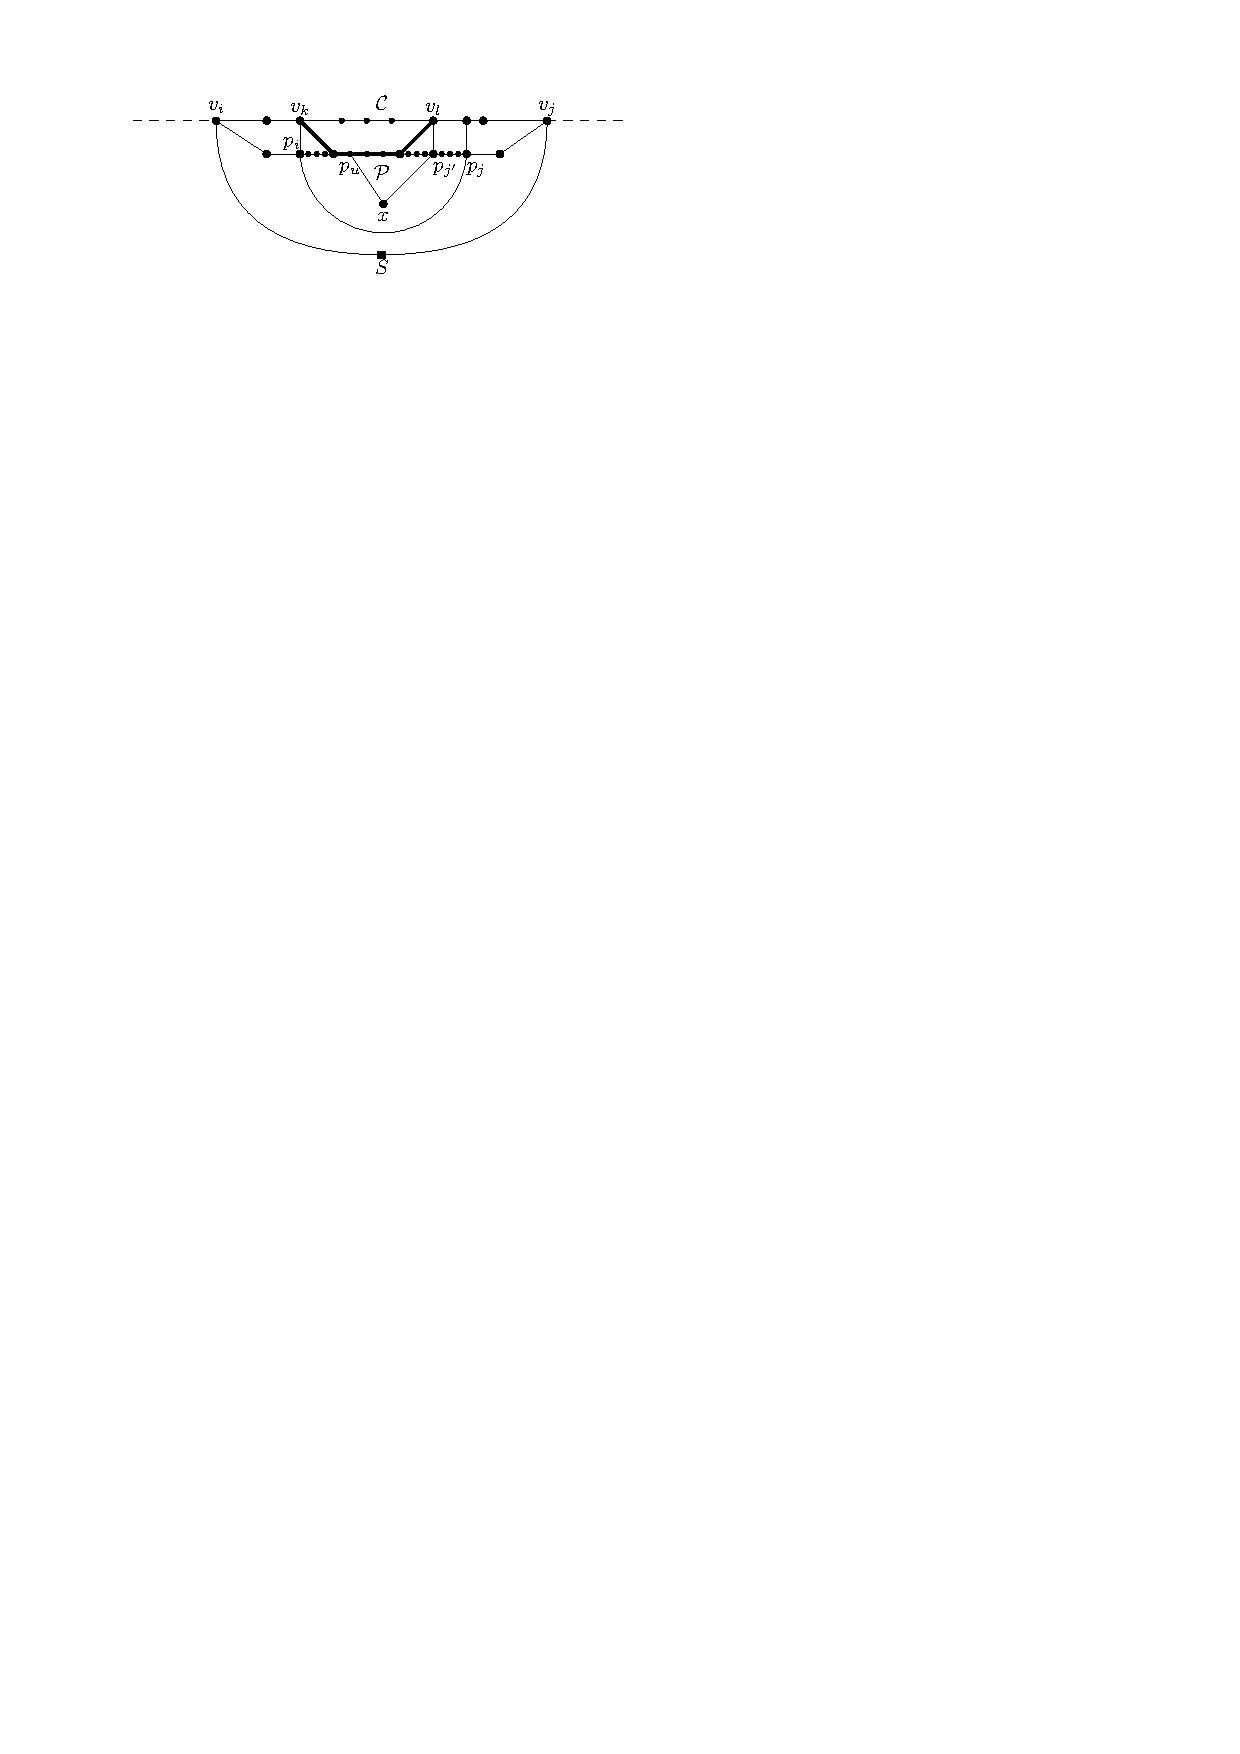
\includegraphics[scale=1]{unifiedAlgo/img/sweep/2chordInChordUpdate}
      \caption{}
      \label{fig:sweep:2chordInChordUpdate}
    \end{figure}

    \paragraph{Only separating 2-chords}
    \emph{Any $\pE$-bound 2-chords}
    Start a path inside the smallest 2-chord (i.e. with the highest starting number for its range). Say the start of this range is $i_1$ we then augment the sweepcycle in the following way.

    Let $v_k$ be the shared neighbor on the sweepcycle of $p_{i_1}$ $p_{i_1 +1}$. We augment the sweepcycle with the right neighbor path of $\cpath|_{v_k, \pE}$. See Figure \ref{fig:sweep:pEBound}.

    \begin{figure}[h]
      \centering
      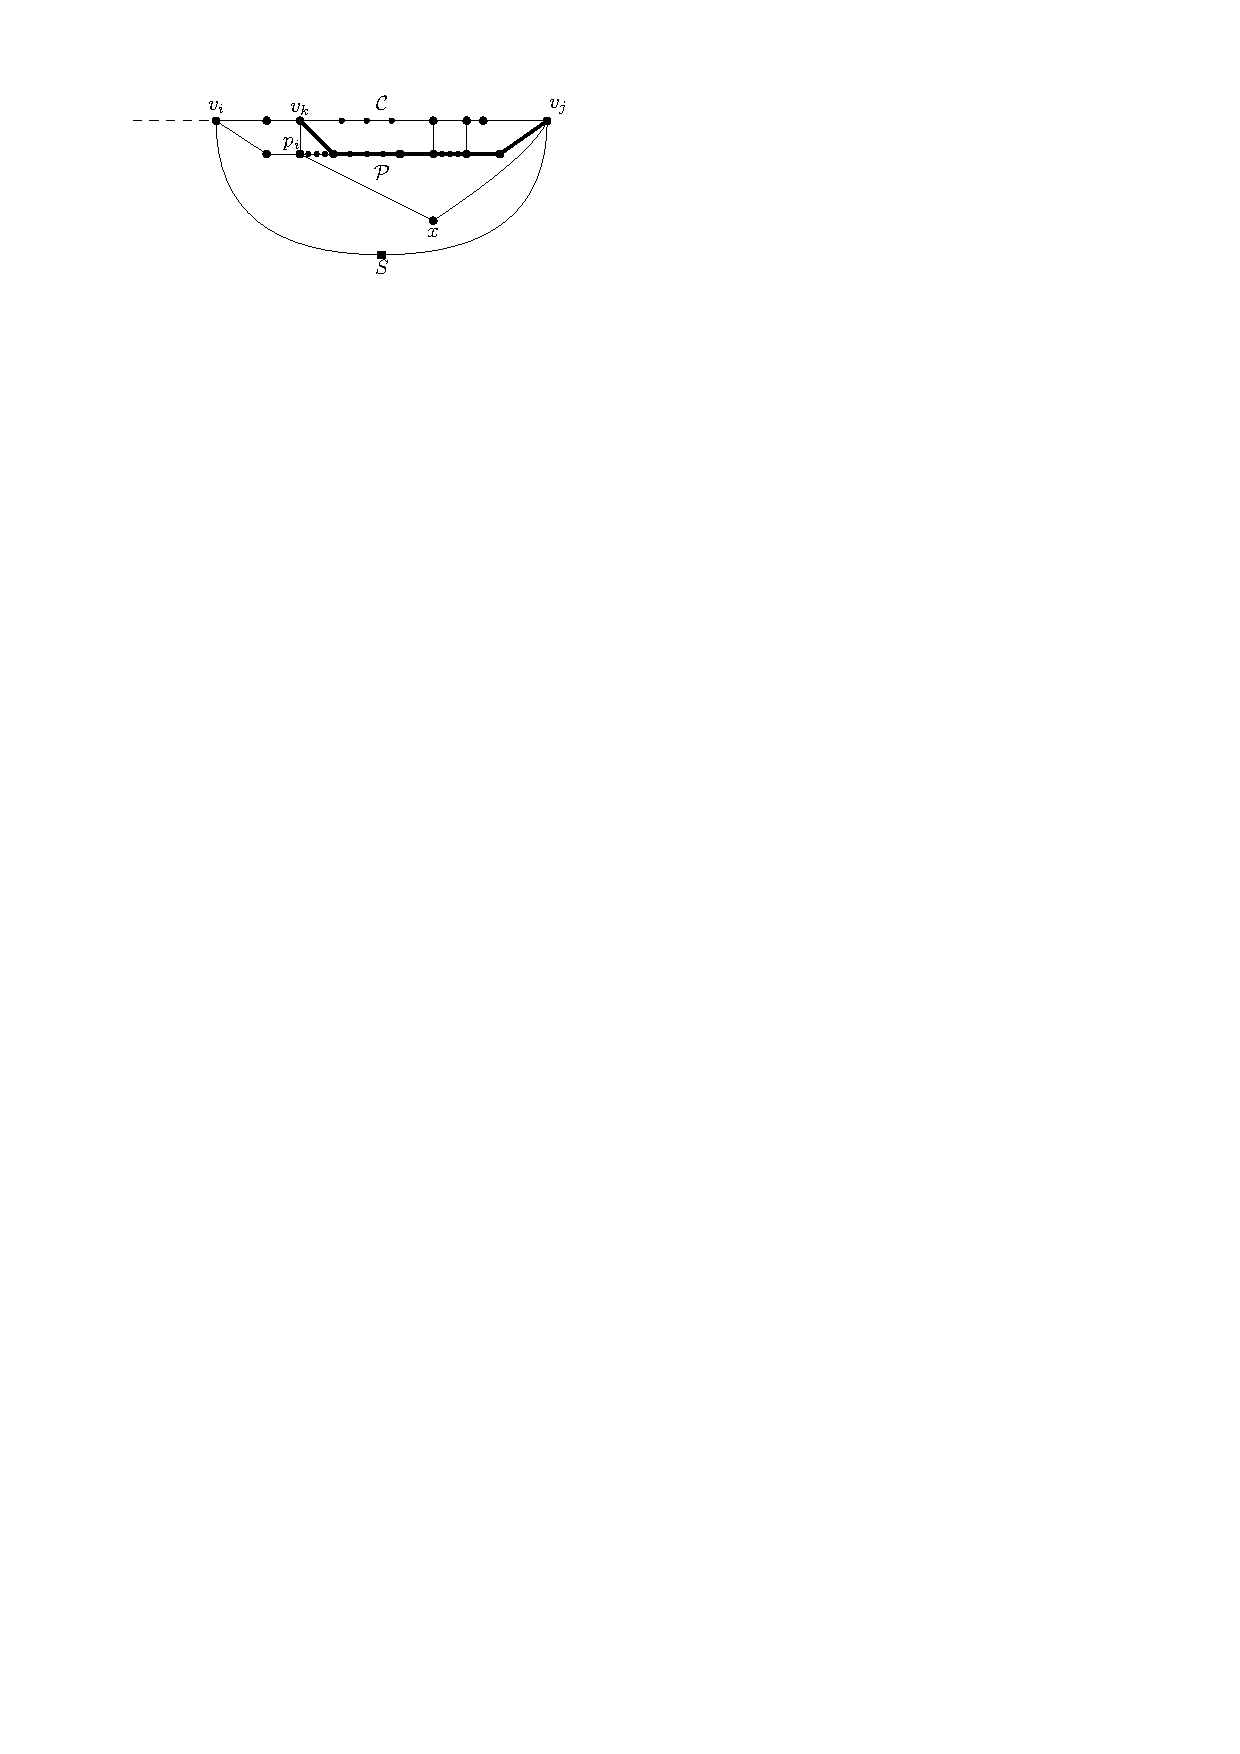
\includegraphics[scale=1]{unifiedAlgo/img/sweep/pEBound}
      \caption{}
      \label{fig:sweep:pEBound}
    \end{figure}
    \emph{Other separating 2-chords}
    The 2-chord can't contain a chord since then we would be in the above case.
    Find the $2$-chord with the lowest end of range. Say that this is $j_1$. We then augment the sweepcycle in the following way.

    Let $v_l$ be the shared neighbor on the sweepcycle of $p_{j_1}$ $p_{j_1 -1}$. We augment the sweepcycle with the right neighbor path of $\cpath|_{v_i, v_l}$. See Figure \ref{fig:sweep:free2chord}.

    \begin{figure}[h]
      \centering
      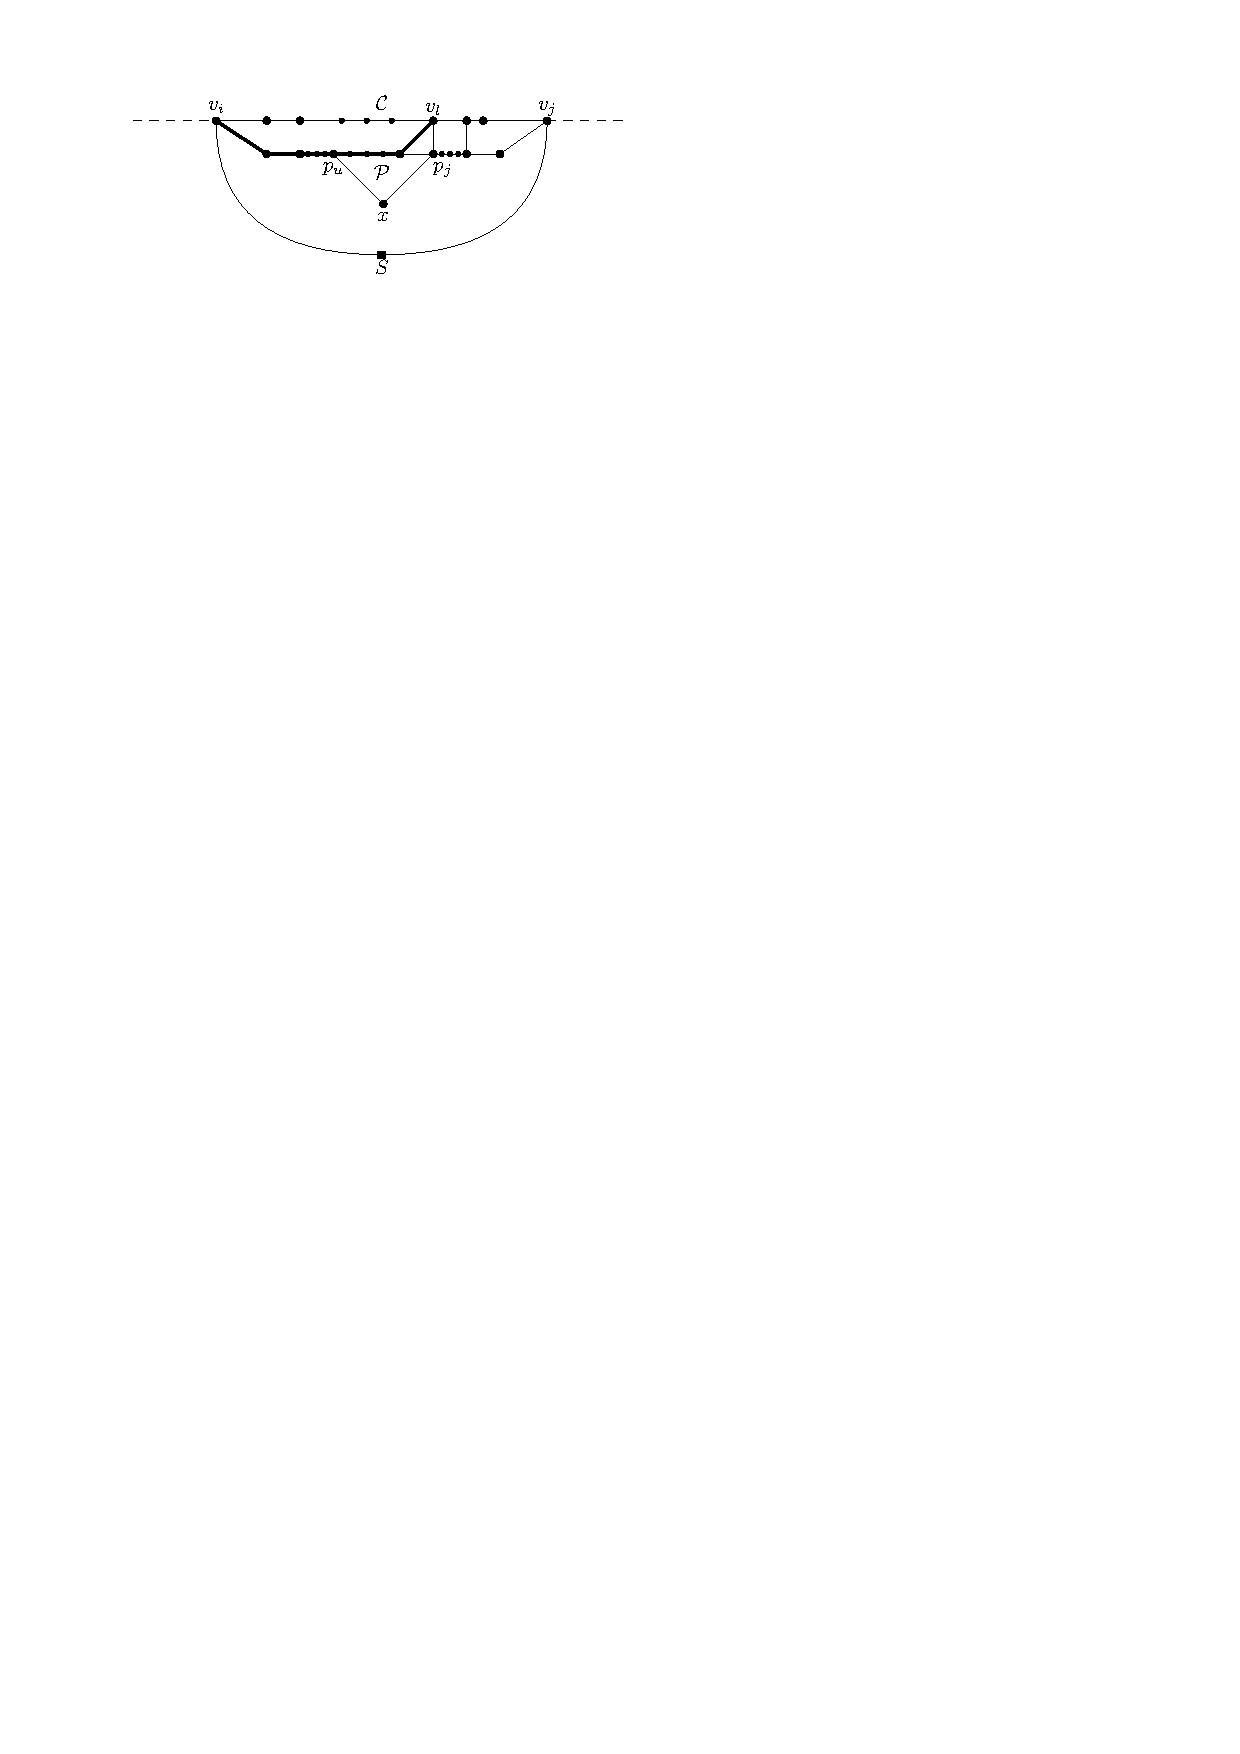
\includegraphics[scale=1]{unifiedAlgo/img/sweep/free2chord}
      \caption{}
      \label{fig:sweep:free2chord}
    \end{figure}

    \paragraph{Augmenting}
      Once we found this augmenting path we augment the sweepcycle with this path. We do this in the following way. We color all interior edge of $\C_\P$ red and orient them towards $\C$. We also color all edges of $\cpath|_{v_i,v_j}$  blue and orient them towards $v_j$. We then update the sweepcycle to $\C'$ by replacing $\cpath|_{v_i,v_j}$ by $\P$.


    \begin{lemma}
      The augmenting paths have no chords or separating $2$-chords
      \label{lm:sweep:augNoIregularity}
    \end{lemma}
    \begin{proof}
        All of these structures are on the right of the augmenting path, since the augmenting path is a subset of a prefence and a  prefence satisfies \ref{p:Wchordfree} (no chords on the left) and \ref{p:noInteriorVertex} (no separating 2-chords on the left).

        If the prefence had any chords the augmenting path is adapted to be entirely inside a chord containing no more chords. Hence the augmenting path can't have any chords.

        Moreover any augmenting path stops before the end of a separating 2-chord unless it is a $\pE$-bound separating 2-chord in which case it only starts after the begin of this 2-chord. Either way the augmenting path also has no separating 2-chords.
    \end{proof}

    \begin{lemma}
      \label{lm:sweep:noConnectingIregularity}
      There are no chords or separating $2$-chords not containing $\pS$ with one endpoint on the old sweepcycle and the other endpoint on the augmenting path.
    \end{lemma}

    \begin{proof}
      \emph{No irregularity}
      Since $v_i$ and $v_j$ are both adjacent to $\pS$ we can't have any chords. And any $2$-chords have $\pS$ as middle vertex. However these are allowed for the Lemma.

      \emph{Chord, not containing a 2-chord}
      Any chord or separating $2$-chord will have to cross $v_k p_i p_j v_l$ so we can't have a chord. Any 2-chord has to have $p_i$ or $p_j$ as middle vertex. But with this restriction the 2-chord can't be separating.

      \emph{Chord, containing a 2-chord}
      In the same manner as in the above case we can't expect any chord or separating 2-chord to connect outside the containing chord.
      Suppose that we have a separating $2$-chord then that would have been a chord of the prefence. This is in contradiction with the fact that the outer chord contained no more chords.
      Suppose that we have a chord not connecting to the second-to-last vertex of the augmenting path. This chord would offend Invariant \ref{i:uni:no2Chords} of the old sweepcycle. Furthermore the second-to-last vertex of the augmenting path has no chords since it would break $v_l p_j x p_u$. (see Figure \ref{fig:sweep:2chordInChordUpdate}).

      \emph{$\pE$-bound separating $2$-chord}
      We can't have any chords since these would have to break $\pE x p_i v_k$. Any $2-chords$ would have $x$ or $p_i$ as middle vertex. However the first yields a $2$-chord of the prefence with a higher start range, this is a contradiction. And the second can't yield an separating $2$-chord.


      \emph{Other separating $2$-chord}
      Any chord or $2$-chord with one vertex in the augmenting path and the other on the old sweepcycle must end to the right of the augmenting path since the augmenting path starts at $\pW$.
      Suppose that we have a separating $2$-chord then that would have been a chord of the prefence. This is in contradiction with the assumption that the prefence had no chords.
      Suppose that we have a chord not connecting to the second-to-last vertex of the augmenting path. This chord would offend Invariant \ref{i:uni:no2Chords} of the old sweepcycle. Furthermore the second-to-last vertex of the augmenting path has no chords since it would break $v_l p_j x p_u$. (see Figure \ref{fig:sweep:free2chord}).
    \end{proof}

    \begin{lemma}
      All five augmenting path types maintain the sweepcycle invariants
    \end{lemma}
    \begin{proof}
      We will proof that the new sweepcycle $\C'$ obtained by augmenting $\C$ is again a valid sweepcycle. Invariant \ref{i:uni:SWandSE} remains trivially true. Invariant \ref{i:uni:intVertCond} hold due to the way we colored the edges around the new interior vertices.

      To see that Invariants \ref{i:uni:noChords} and \ref{i:uni:no2Chords} still hold note that due to prefence Property \ref{p:Cchordfree} and the fact that the augmenting path itself has no irregularities (Lemma \ref{lm:sweep:augNoIregularity})
      we know any $(2-)$chord $C$ has to have one vertex on $\P$ and one vertex on the unchanged part of old sweepcyle $\C \cap C'$. However these potential chords are also not offending by Lemma \ref{lm:sweep:noConnectingIregularity}.

      Hence $\C'$ is a valid new sweepcycle.
    \end{proof}

    \begin{lemma}
      \label{lm:sweep:REL}
      The resulting structure is a REL
    \end{lemma}

    \begin{proof}
      \fxnote{We should patch up the last step. That is, what to do when the sweepcycle is no longer separating }
      After running the whole algorithm the interior vertex condition holds for all vertices in the graph. Furthermore the poles are also colored correctly due to Invariant \ref{i:uni:SWandSE}.
    \end{proof}

    Given a splitvertex $v$ we will by \emph{bottom} path mean the path that comes in trough the first incoming blue edge in the the rotation at $v$ and leaves through the last outgoing blue edge in the rotation at $v$. See Figure \ref{fig:sweep:bottomPath}.

    \begin{figure}[h]
      \centering
      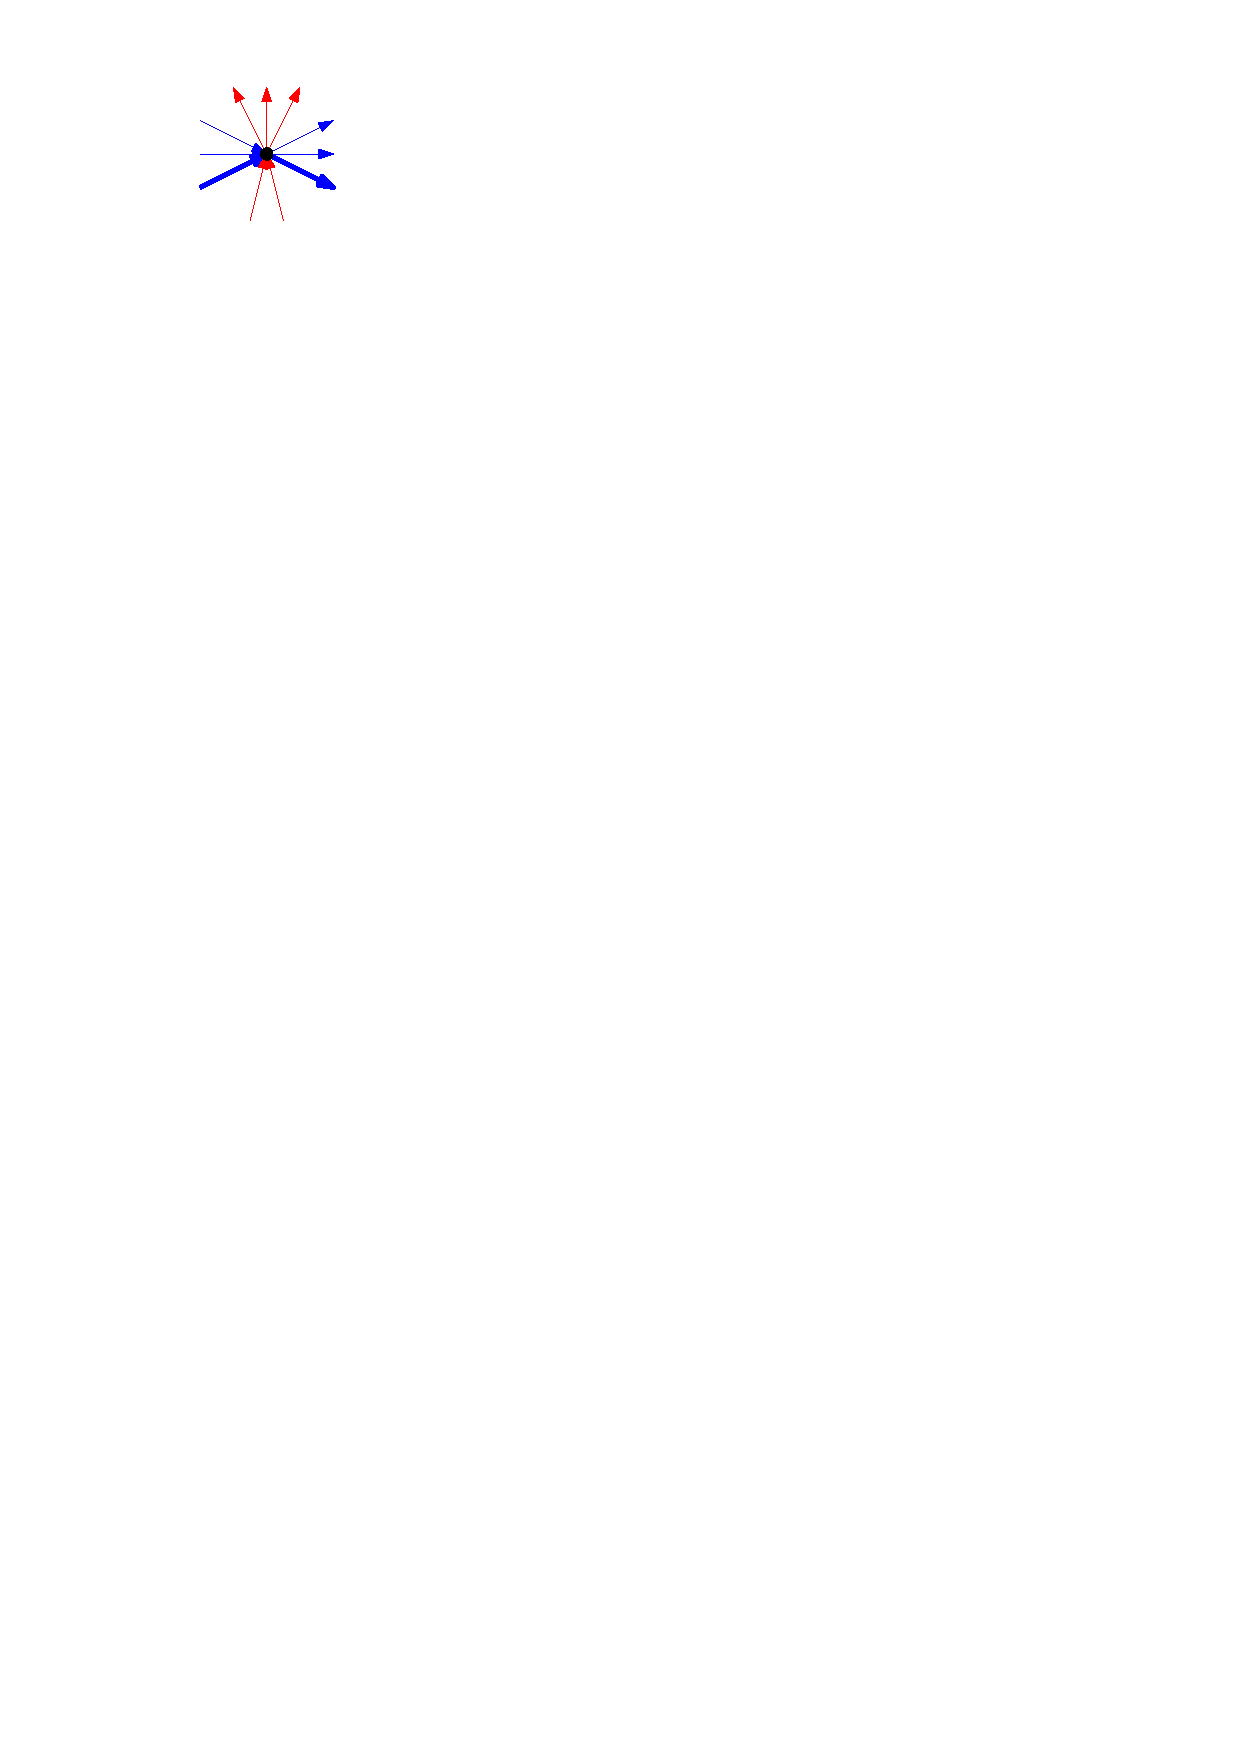
\includegraphics[scale=1]{unifiedAlgo/img/sweep/bottompath.pdf}
      \caption{The bottom path of this splitvertex is given in bold}
      \label{fig:sweep:bottomPath}
    \end{figure}

    \begin{lemma}
      \label{lm:sweep:NoTwoSplitsAboveEachOther}
      Let $v$ be any splitvertex. Then the subsequent vertex on the bottom path $w$ can't be the handle of a large topfan.
    \end{lemma}

    \begin{proof}
      \fxnote{Try to clear up reasoning furthera}
      Note that if $v$ is a splitvertex because it is adjacent to $\pS$ then since $w$ is on the bottom path it also has to be adjacent to $\pS$ by the definition of the bottom path.
      Hence $w$ is not the handle of a large topfan in this case.

      On the other hand if $v$ is a splitvertex due to a chord $v a b x$ we can continue the bottom path past $w$ as an bottom path that will eventually go to $x$. By the way we treat chords in the algorithm. \fxnote{Formalize: "By the way we treat chords"} We will denote this extended bottom path by $\P$. The situation is depicted in Figure \ref{fig:botomPathChord}.

      \begin{figure}[h]
        \centering
        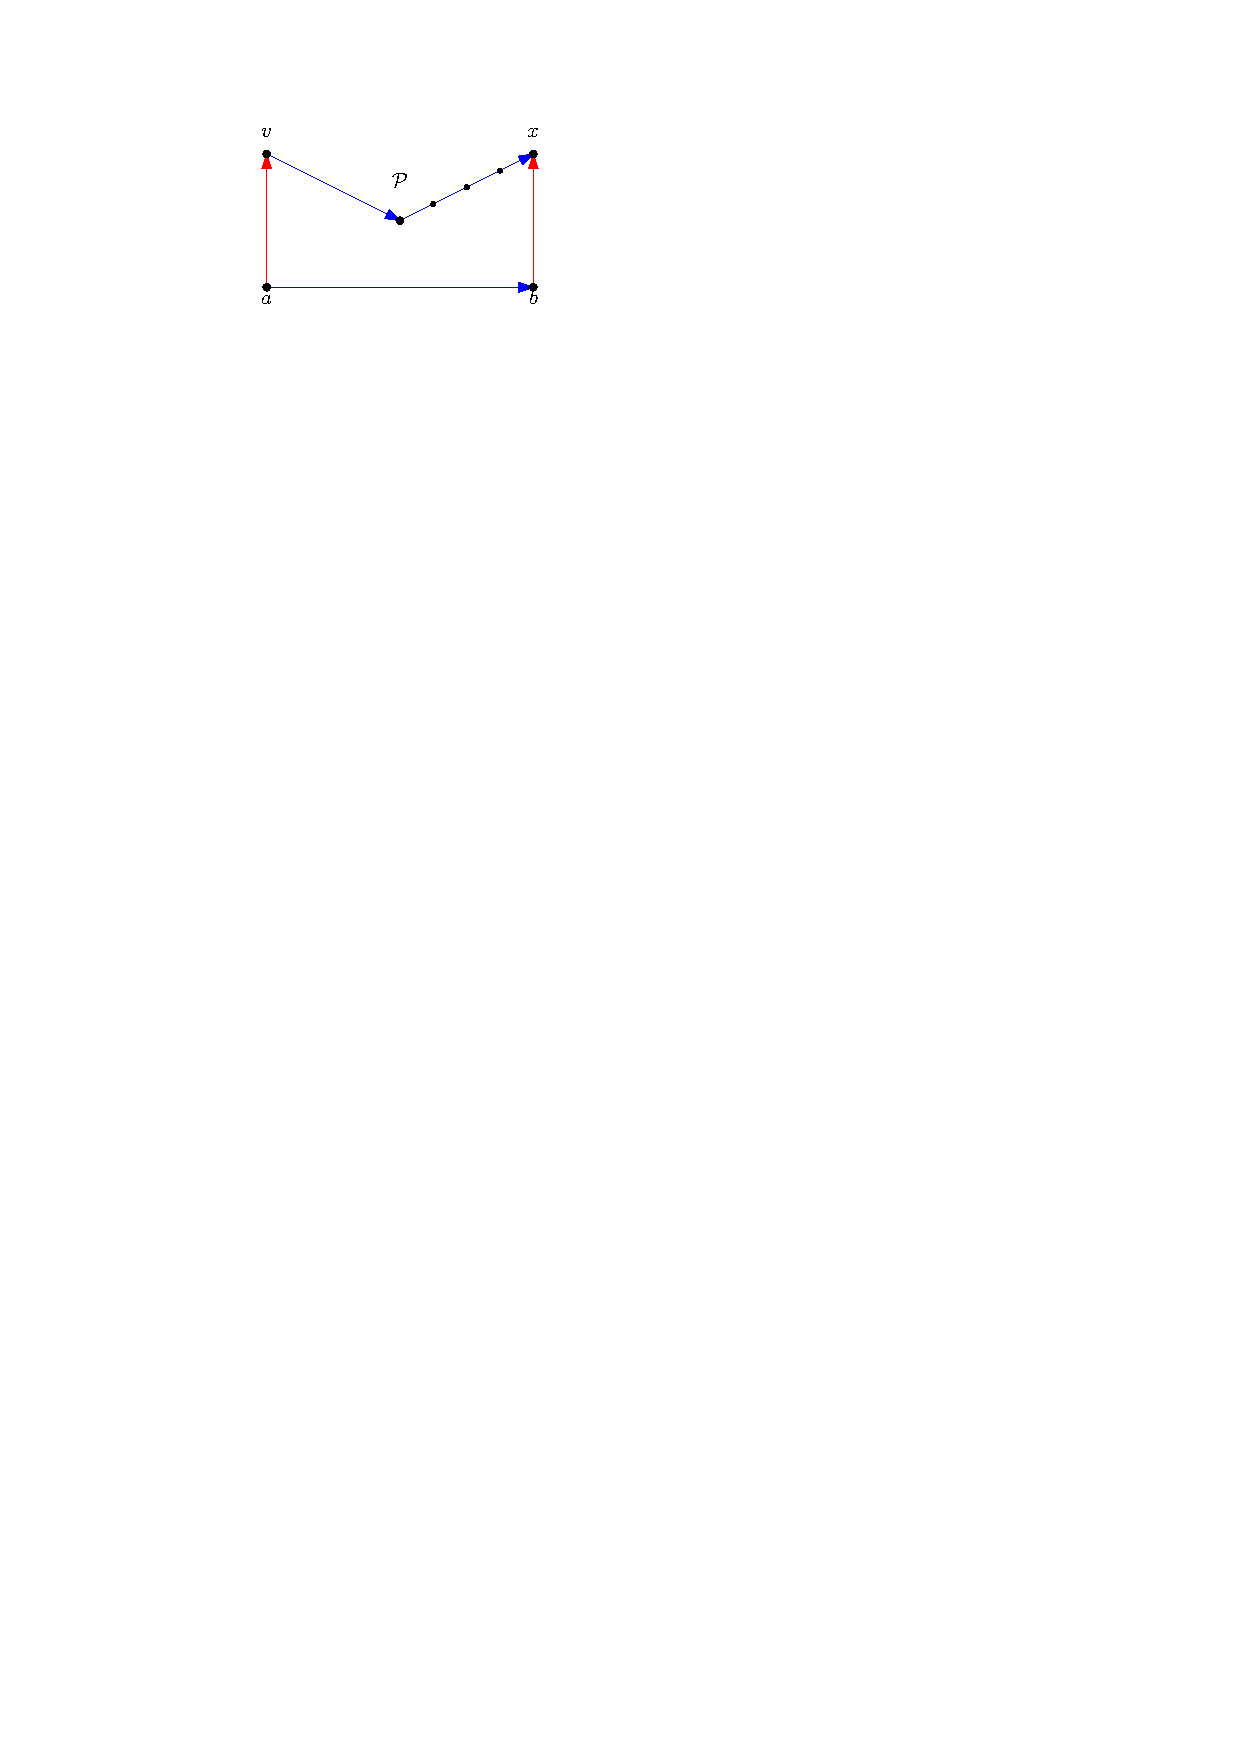
\includegraphics[scale=1]{unifiedAlgo/img/sweep/bottompathChord.pdf}
        \caption{}
        \label{fig:botomPathChord}
      \end{figure}

      The interior of  $vabx \oplus \rev \P$ and has no vertices. Suppose there would be such a vertex then since $\P$ is a bottom path the blue path going trough this vertex has to start at $a$ and end at $b$. But then this gives a blue face with only one edge on it's bottom boundary path, hence the interior of this face has no incoming red edges. \fxnote{Or i could make a lemma about face borders somewhere and contradict with that.} So the result is not a \rel. Since our graph is a \rel $vabx \oplus \rev \P$ has no interior vertices.

      This also implies all interior edges are red (by the definition of bottom path) and thus that $ab$ is blue otherwise we would get a monocolored triangle.

      Now $w$ can't be connected to any vertex in $\P$ that would give a chord. And we don't allow chords in any valid path on the moment we add it. So $w$ can only be connected to $a$ and $b$ and is thus a topfan of size at most $2$. (If it's a topfan at all, since we don't consider topfans of size 1 as topfans.)
    \end{proof}

\newpage
\section{Flipping Blue $Z$'s}
    The \rel provided by the algorithm so far is vertically one-sided in most cases but not always. In the case that this \rel is not one-sided there must be a blue $Z$ (see Figure \ref{fig:zflip:blueZ})

    \begin{figure}[h]
      \centering
      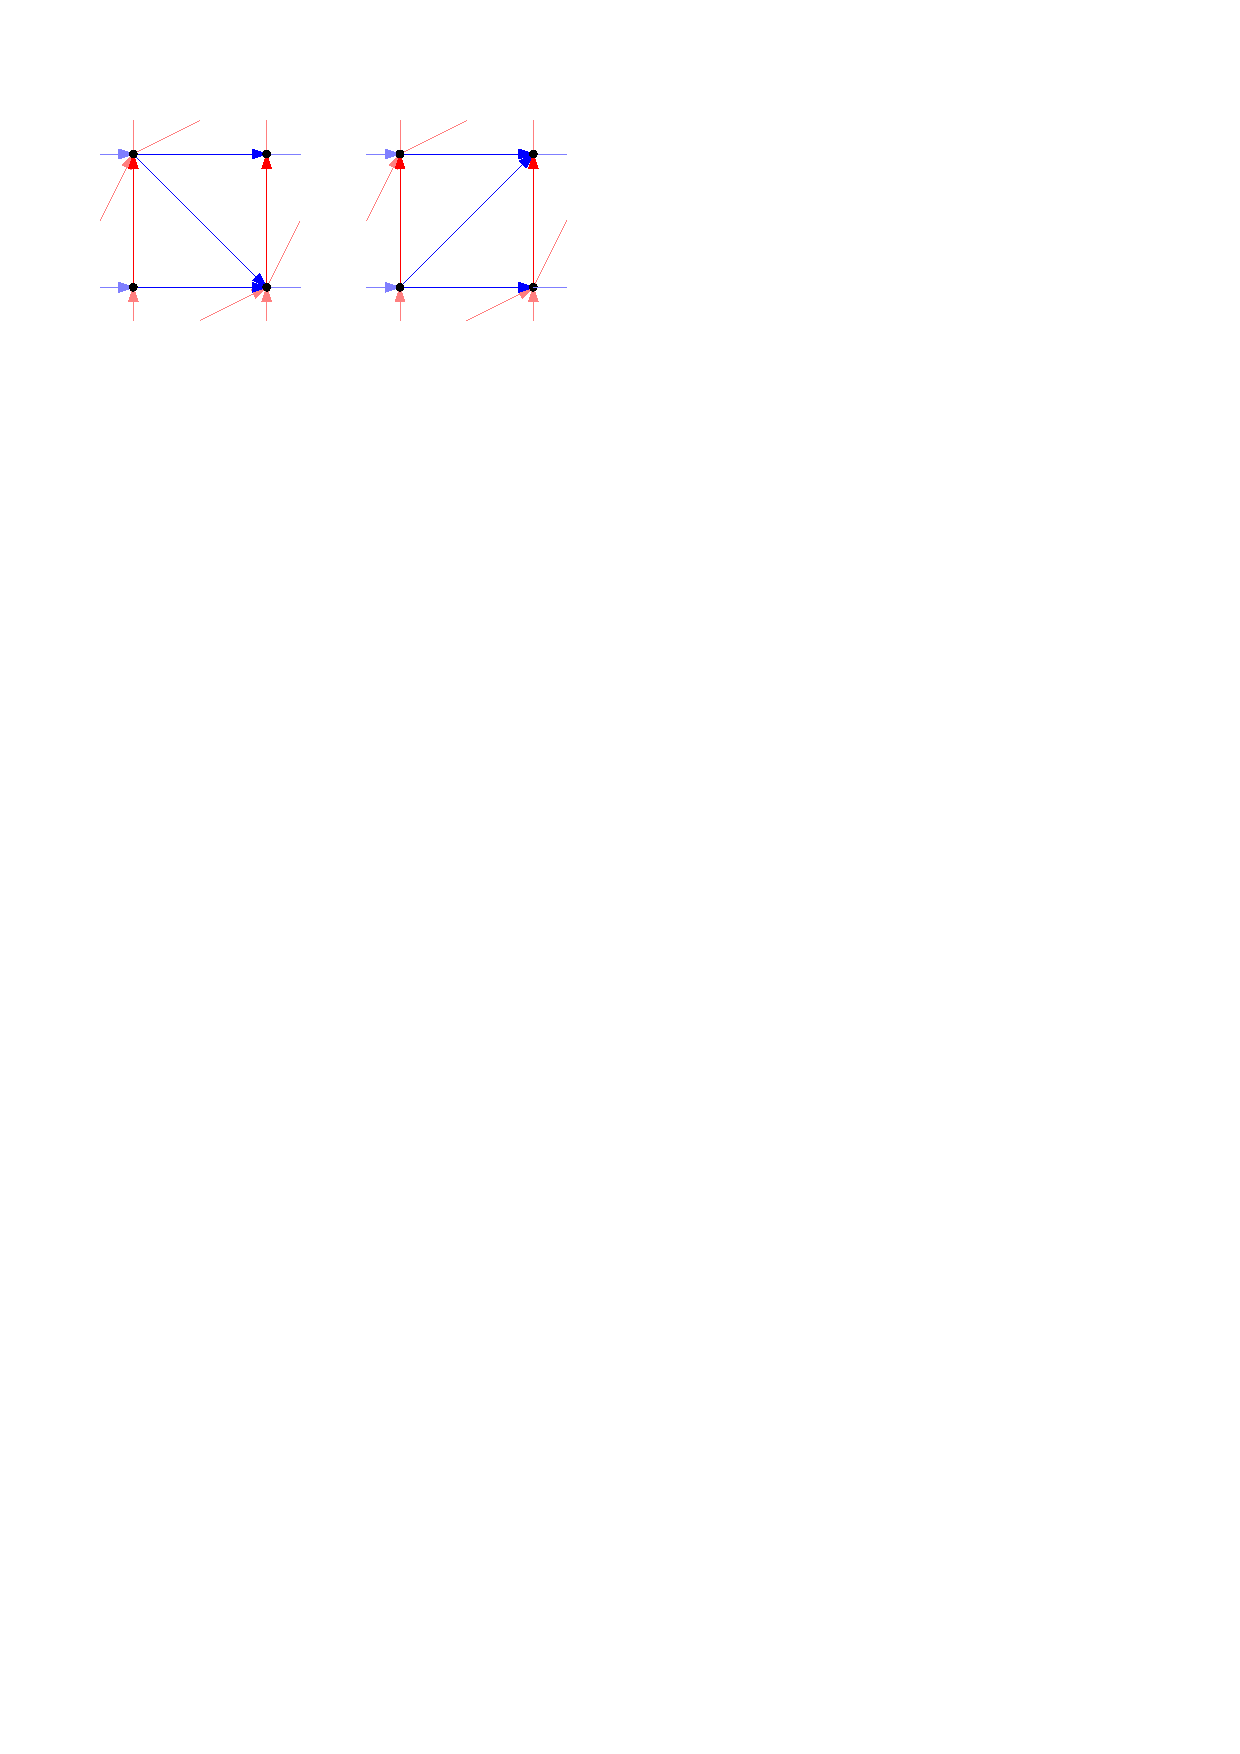
\includegraphics[scale=1]{unifiedAlgo/img/zflip/blueZ.pdf}
      \caption{The two possible blue $Z$'s}
      \label{fig:zflip:blueZ}
    \end{figure}

    We will say that such a $Z$ consists of a \emph{top}, \emph{bottom} and \emph{midlle} edge in straightforward manner. \fxnote{I have some introduction on this subject somewhere}


    As long as the \rel is not vertically one-sided we find such a blue $Z$ and recolor it's middle edge as in Figure \ref{fig:zflip:flip}. We will say that this edge is \emph{flipped}

    Note that both flips transfer one valid \rel to another valid \rel. If the interior vertex condition was fulfilled in Figure \ref{fig:zflip:blueZ} then it is also fulfilled in Figure \ref{fig:zflip:flip}.

     We do this until the \rel is vertically one-sided. Since every flip reduces the number of blue edges by one this is a finite procedure.

    \begin{figure}[h]
      \centering
      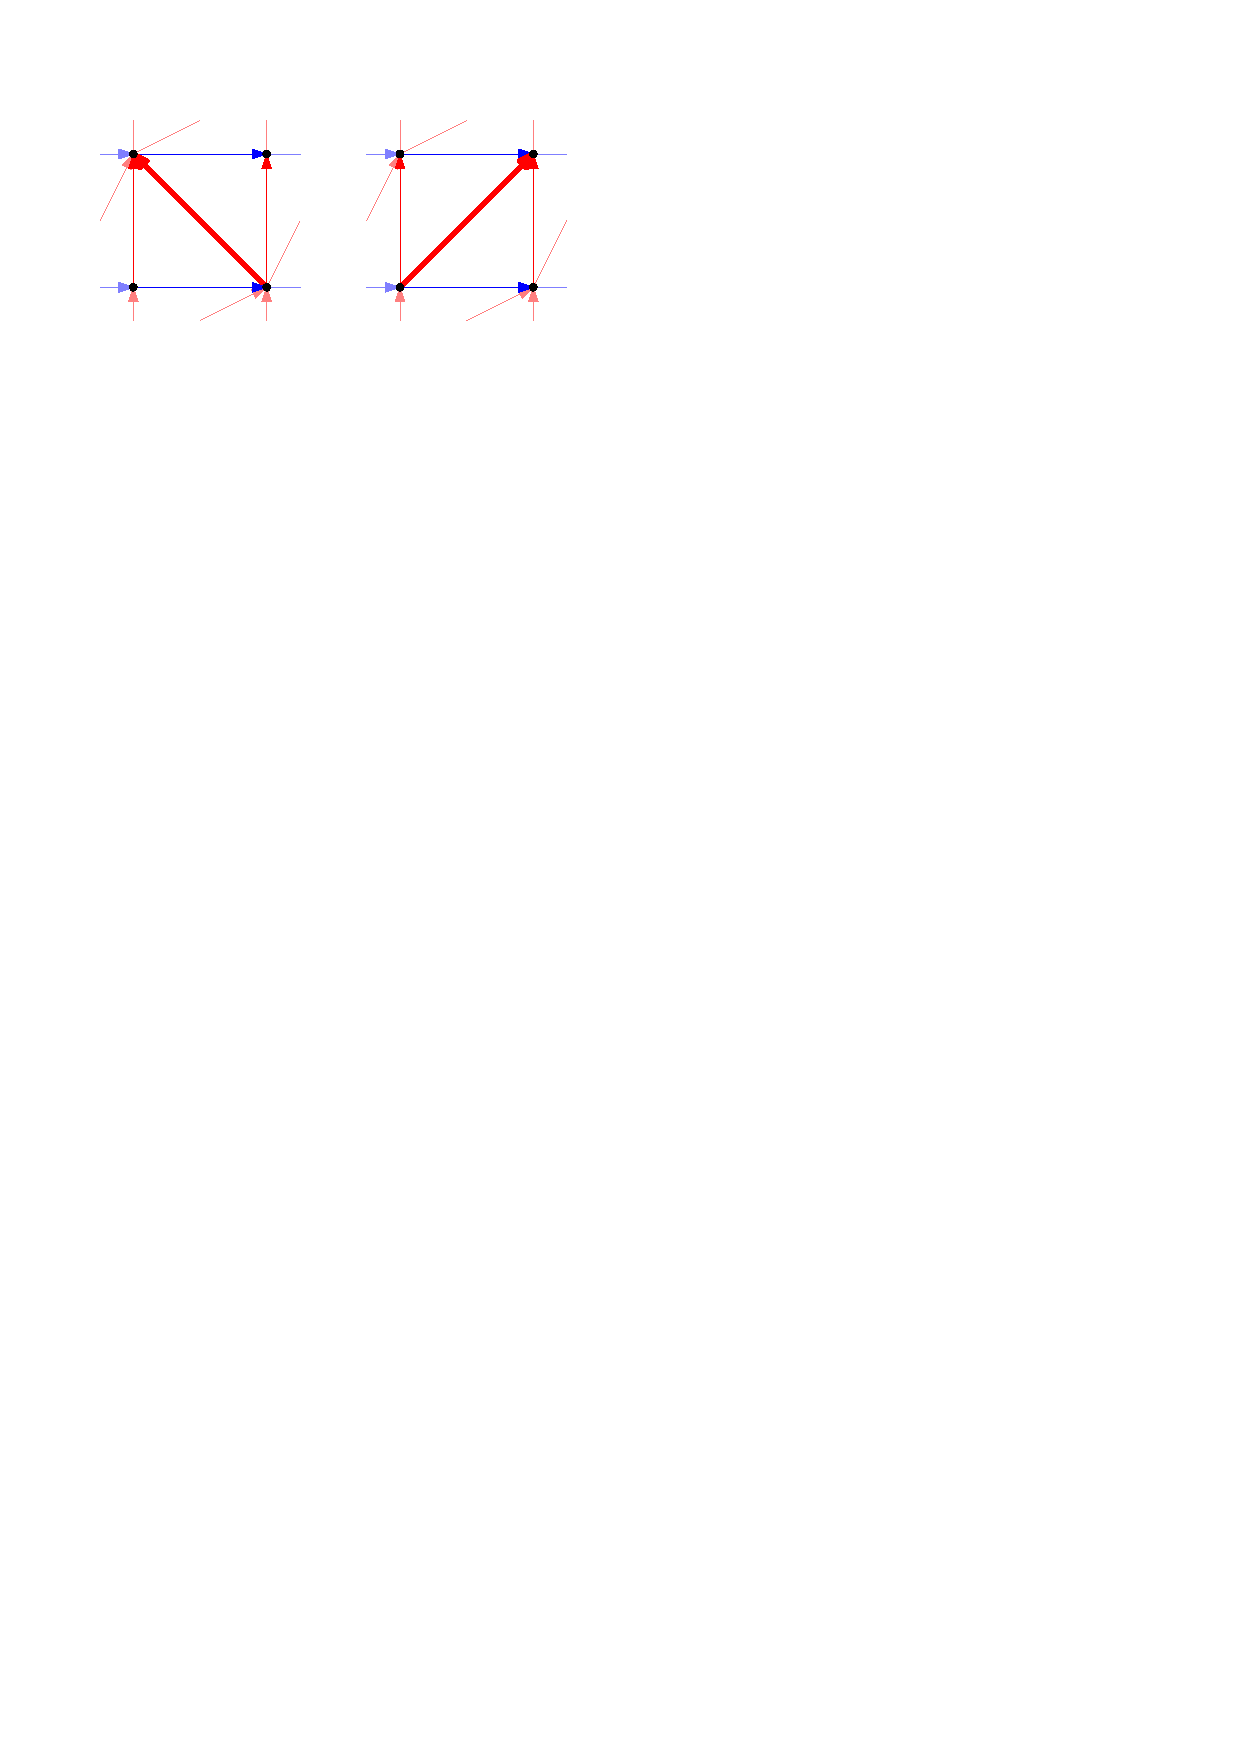
\includegraphics[scale=1]{unifiedAlgo/img/zflip/flip.pdf}
      \caption{The flip}
      \label{fig:zflip:flip}
    \end{figure}

    \begin{lemma}
      \label{lm:sweep:vertOnsided}
      The resulting REL is vertically one-sided
    \end{lemma}
    \begin{proof}
      By construction we flip all blue $Z$'s. If we don't have any more $Z$'s then the remaining \rel is vertically one-sided. \fxnote{refer to some lemma?}
    \end{proof}

    \begin{lemma}
      \label{lm:sweep:NoTwoSplitsAboveEachOtherVertOnesided}
      Lemma \ref{lm:sweep:NoTwoSplitsAboveEachOther} still holds.
    \end{lemma}

    \begin{proof}
      Flipping middle edges of these $Z$'s  can only reduce the number of split vertices.

      For a split vertex $v$ adjacent to $\pS$ we can note that the edge $vw$ will not be flipped because it can't be a middle edge. Hence $w$ is still on the bottom path and still not the handle of a big topfan.

      If $v$ is a split vertex due to a chord let us note the following.
      The edges of $\P$ and $ab$ can't have been flipped since then we would find a monocolored red triangle while a flip leads to another valid \rel. Hence $w$ is still on the bottom path trough $v$ and still can't be the handle of a large topfan.
    \end{proof}

    \fxnote{do we need this to complete the proof? I currently do use it}
    \begin{lemma}
      \label{lm:uni:noTfan above whole path}
      The resulting REL never has a red $T$-fanhandle connected to both split and merge vertex of the same path. Unless the split is $\pS$-adjecent
    \end{lemma}
    \begin{proof}
        This would give a non-trivial separating $5$-cycle. Whether we consider a chord or a polebound 2-chord.
    \end{proof}
